% Figure 24. A complete nonprojective variety (printed page 443).
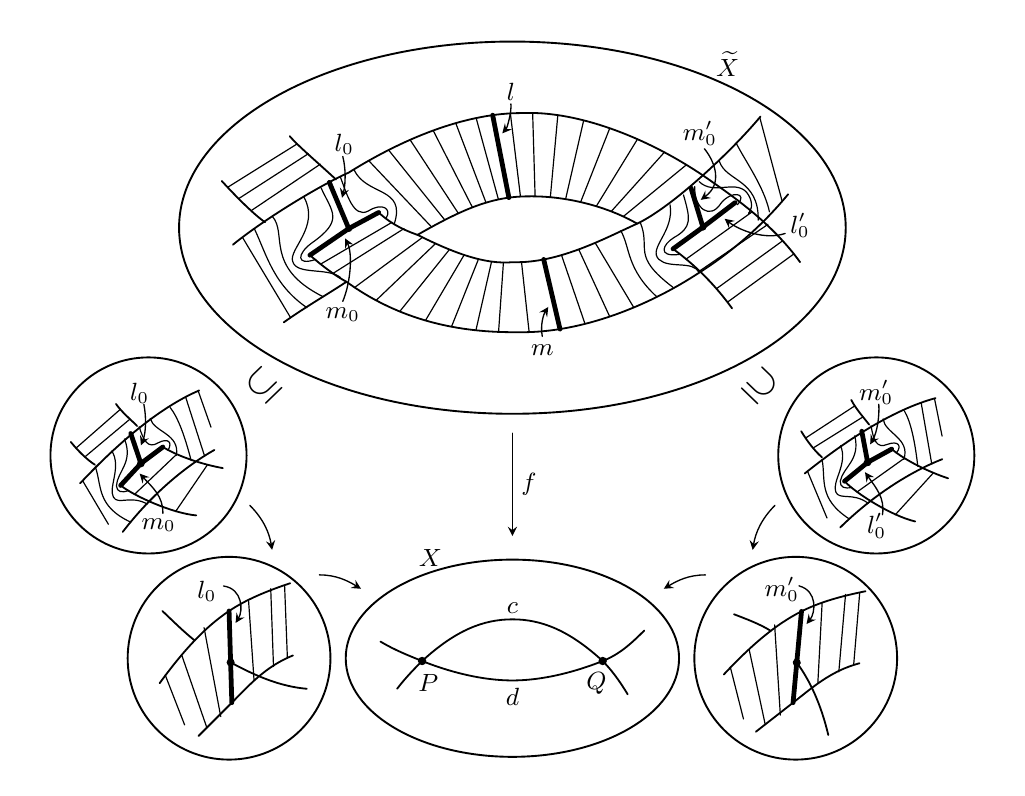
\begin{tikzpicture}[
    x=1bp, y=-1bp, line cap=round, line join=round, >=stealth,
    frame/.style={line width=.68bp},
    edge/.style={line width=.65bp},
    ruling/.style={line width=.43bp},
    fiber/.style={line width=1.72bp},
    leader/.style={->,line width=.48bp},
    every node/.style={font=\small,inner sep=0pt}
  ]
  \path[use as bounding box] (0,0) rectangle (349,266.4);

  \draw[frame] (174.5,72) ellipse[x radius=120, y radius=67];
  \draw[frame] (43.5,154) circle[radius=35.3];
  \draw[frame] (305.5,154) circle[radius=35.3];
  \draw[frame] (72.5,227) circle[radius=36.5];
  \draw[frame] (276.5,227) circle[radius=36.5];
  \draw[frame] (174.5,227) ellipse[x radius=60, y radius=35.5];

  % The two local views lie in the variety at the top.
  \node[rotate=44,font=\Large] at (85,129) {$\subseteq$};
  \node[rotate=-44,font=\Large] at (264,129) {$\supseteq$};
  \node at (252,13) {$\widetilde X$};

  % The ruled surface in the top view and its two local crossings.
  \begin{scope}[shift={(66.9,18.9)}, x=.269bp,y=-.252bp]
    \coordinate (back-left) at (181,132);
    \coordinate (back-right) at (667,145);
    \coordinate (front-left) at (178,288);
    \coordinate (front-right) at (650,275);
    \coordinate (inside-left) at (273,221);
    \coordinate (inside-right) at (567,205);
    \coordinate (left-junction) at (181,212);
    \coordinate (right-junction) at (655,210);

    % The four edges of the front and back bands.
    \draw[edge] (26,235)
      .. controls (70,197) and (143,150) .. (back-left)
      .. controls (262,78) and (343,47) .. (412,47)
      .. controls (495,43) and (595,90) .. (back-right);
    \draw[edge] (94,346)
      .. controls (123,324) and (151,307) .. (front-left)
      .. controls (250,344) and (330,361) .. (407,360)
      .. controls (492,362) and (583,322) .. (front-right)
      .. controls (691,247) and (732,211) .. (769,163);
    \draw[edge] (inside-left)
      .. controls (332,185) and (372,166) .. (421,166)
      .. controls (473,165) and (528,181) .. (inside-right);
    \draw[edge] (inside-left)
      .. controls (318,245) and (362,264) .. (401,260)
      .. controls (463,262) and (527,224) .. (inside-right)
      .. controls (614,181) and (693,102) .. (732,52);

    \draw[ruling]
      (207.7,115.0) -- (291.8,209.7)
      (234.3,99.8) -- (309.5,199.7)
      (263.1,85.2) -- (327.7,190.3)
      (294.0,71.9) -- (346.5,181.7)
      (324.2,61.4) -- (364.7,175.0)
      (351.5,54.1) -- (381.3,170.4)
      (397.3,47.5) -- (410.8,166.3)
      (427.1,46.8) -- (430.4,166.0)
      (460.8,49.9) -- (450.8,167.2)
      (495.4,57.4) -- (471.2,170.0)
      (530.3,68.7) -- (491.3,174.2)
      (567.4,84.3) -- (512.3,180.1)
      (603.4,103.0) -- (532.3,187.5)
      (632.9,120.9) -- (548.4,194.8)
      (188.9,296.1) -- (279.7,224.6)
      (217.6,314.6) -- (297.2,233.4)
      (249.2,330.5) -- (315.8,241.9)
      (283.7,343.3) -- (335.4,249.7)
      (318.5,352.2) -- (354.6,255.6)
      (351.2,357.3) -- (372.1,259.2)
      (381.5,359.6) -- (388.0,260.5)
      (422.4,359.9) -- (412.2,259.9)
      (497.2,348.2) -- (465.7,249.9)
      (530.2,337.7) -- (488.8,241.8)
      (562.4,324.7) -- (510.8,232.4);

    % Left patch. The diagonal strip is interrupted at the crossing.
    \draw[edge]
      (11,144) .. controls (29,165) and (53,191) .. (69,203)
      (102,80) .. controls (113,94) and (142,120) .. (164,142)
      (129,250) .. controls (145,265) and (165,281) .. (front-left)
      (221,189) .. controls (234,202) and (249,212) .. (inside-left);
    \draw[ruling]
      (19,153) -- (112,91)
      (34,169) -- (127,105)
      (51,186) -- (143,120)
      (143,263) -- (239,203)
      (160,276) -- (255,212)
      (39,225) -- (103,339)
      (55,213) .. controls (71,249) and (80,292) .. (125,325)
      (79,195) .. controls (99,219) and (68,267) .. (146,309)
      (121,167) .. controls (143,209) and (100,242) .. (106,259)
        .. controls (111,279) and (153,267) .. (170,282)
      (144,154) .. controls (159,189) and (175,200) .. (131,233)
        .. controls (112,248) and (110,266) .. (137,256)
      (170,139) .. controls (178,161) and (187,198) .. (207,187)
        .. controls (226,174) and (239,184) .. (231,197)
      (188,128) .. controls (205,166) and (258,152) .. (242,205);
    \draw[fiber]
      (155,146) -- (left-junction)
      (129,250) -- (left-junction) -- (221,189);
    \fill (left-junction) circle[radius=1.25bp];

    % Right patch, with the roles of the two fibers interchanged.
    \draw[edge]
      (back-right) .. controls (702,171) and (750,208) .. (785,260)
      (615,241) .. controls (647,266) and (673,295) .. (694,326);
    \draw[ruling]
      (632,256) -- (721,188)
      (650,273) -- (742,206)
      (673,298) -- (761,230)
      (688,317) -- (777,248)
      (731,53) -- (761,173)
      (700,91) .. controls (712,116) and (737,153) .. (744,188)
      (677,116) .. controls (686,145) and (730,141) .. (729,200)
      (650,145) .. controls (670,166) and (702,139) .. (716,164)
        .. controls (724,179) and (718,188) .. (716,190)
      (644,152) .. controls (643,184) and (665,200) .. (679,176)
        .. controls (693,157) and (716,161) .. (701,178)
      (629,164) .. controls (638,198) and (641,210) .. (616,225)
        .. controls (602,234) and (593,253) .. (623,249)
      (611,178) .. controls (617,217) and (581,240) .. (596,256)
        .. controls (610,270) and (642,257) .. (650,275)
      (571,203) .. controls (586,241) and (558,250) .. (615,296)
      (545,215) .. controls (558,239) and (552,269) .. (593.4,309.6);
    \draw[fiber]
      (639,154) -- (right-junction)
      (615,241) -- (right-junction) -- (698,175);
    \fill (right-junction) circle[radius=1.25bp];

    \draw[fiber]
      (373.6,50.0) -- (395.3,167.8)
      (463.7,355.6) -- (441.9,256.1);
    \node at (398,16) {$l$};
    \draw[leader] (398,34) .. controls (399,46) and (393,68) .. (386.5,76);
    \node at (440,385) {$m$};
    \draw[leader] (440,366) .. controls (437,349) and (442,334) .. (448,324);
    \node at (175,92) {$l_0$};
    \draw[leader] (173,109) .. controls (177,125) and (177,148) .. (172,168);
    \node at (173,335) {$m_0$};
    \draw[leader] (173,316) .. controls (184,288) and (186,247) .. (176,226);
    \node at (651,76) {$m'_0$};
    \draw[leader] (657,98) .. controls (672,118) and (681,148) .. (652,171);
    \node at (785,208) {$l'_0$};
    \draw[leader] (765,219) .. controls (738,229) and (703,214) .. (684,198);
  \end{scope}

  % The two intermediate views share the local geometry, with exchanged labels.
  \def\DrawDoublePatch#1#2{%
    \begin{scope}[x=.152bp,y=-.152bp]
      \begin{scope}[shift={(-218,-218)}]
        \coordinate (junction) at (200,237);
        \draw[edge]
          (56,284) .. controls (112,225) and (222,114) .. (338,64)
          (157,399) .. controls (223,313) and (303,245) .. (374,205)
          (34,186) .. controls (49,205) and (72,228) .. (91,240)
          (141,96) .. controls (154,115) and (179,136) .. (191,148)
          (152,289) .. controls (185,315) and (275,355) .. (331,360)
          (252,198) .. controls (291,222) and (350,240) .. (394,248);
        \draw[ruling]
          (47,200) -- (151,109)
          (69,220) -- (174,132)
          (185,310) -- (284,216)
          (282,351) -- (357,241)
          (62,278) -- (123,381)
          (92,245) .. controls (108,290) and (94,338) .. (176,376)
          (131,207) .. controls (155,246) and (122,294) .. (135,317)
            .. controls (146,336) and (175,311) .. (215,333)
          (161,179) .. controls (183,234) and (144,256) .. (142,290)
            .. controls (143,305) and (155,307) .. (171,301)
          (196,150) .. controls (206,183) and (217,203) .. (241,188)
            .. controls (264,176) and (276,186) .. (264,206)
          (222,130) .. controls (230,163) and (293,166) .. (284,218)
          (269,104) .. controls (288,128) and (304,172) .. (319,230)
          (306,80) -- (351,220)
          (336,66) -- (366,151);
        \draw[fiber]
          (176,166) -- (junction)
          (152,289) -- (junction) -- (252,198);
        \fill (junction) circle[radius=1.4bp];
        \node at (197,71) {$#1$};
        \draw[leader] (207,97) .. controls (213,126) and (212,164) .. (200,194);
        \node at (242,383) {$#2$};
        \draw[leader] (252,355) .. controls (253,315) and (227,293) .. (197,261);
      \end{scope}
    \end{scope}%
  }
  \begin{scope}[shift={(43.5,154)}]
    \DrawDoublePatch{l_0}{m_0}
  \end{scope}
  \begin{scope}[shift={(305.5,154)},rotate=-8]
    \DrawDoublePatch{m'_0}{l'_0}
  \end{scope}

  % The first blow-up in each neighborhood, before the second curve is blown up.
  \def\DrawFirstPatch#1#2{%
    \coordinate (on-fiber) at (.56,1.5);
    \draw[edge]
      (-25,9) .. controls (-17,-2) and (-9,-11) .. (0,-17)
        coordinate[pos=.52] (left-entry) coordinate[pos=.61] (right-entry)
        .. controls (6,-21) and (13,-24) .. (22,-27)
      (-11,28) .. controls (-7,24) and (-3,20) .. (1,16)
        .. controls (7,10) and (13,3) .. (23,-1);
    % Only the parts of the transverse curve visible past the band are drawn.
    \draw[edge] #2;
    \draw[ruling]
      (-23,6) -- (-16,24)
      (-17,-1) -- (-8,25)
      (-9,-11) -- (-3,21)
      (7,-21) -- (9,8)
      (15,-25) -- (16,3)
      (20,-26) -- (21,0);
    \draw[fiber] (0,-17) -- (1,16);
    \fill (on-fiber) circle[radius=1.45bp];
    \node at (-8,-24) {$#1$};
    \draw[leader] (-2,-26) .. controls (5,-25) and (5,-17) .. (2.35,-12.7);
  }
  \begin{scope}[shift={(72.5,227)}]
    \DrawFirstPatch{l_0}{
      (-24,-17) .. controls (-20.1,-13.3) and (-16.4,-9.6) .. (left-entry)
      (on-fiber) .. controls (9.6,6.4) and (18.5,10.2) .. (28,11)
    }
  \end{scope}
  \begin{scope}[shift={(276.5,227)},rotate=-7]
    \DrawFirstPatch{m'_0}{
      (-24,-13) .. controls (-20,-12) and (-14,-10.6) .. (right-entry)
      (on-fiber) .. controls (6,7.3) and (11,15.2) .. (15,26)
    }
  \end{scope}

  % The four local maps and the global map f.
  \draw[leader] (80,172) .. controls (85,177) and (87,182) .. (88,188);
  \draw[leader] (269,172) .. controls (264,177) and (262,182) .. (261,188);
  \draw[leader] (105,197) .. controls (111,197) and (115,199) .. (120,202);
  \draw[leader] (244,197) .. controls (238,197) and (234,199) .. (229,202);
  \draw[leader] (174.5,146) -- node[right=3bp] {$f$} (174.5,183);

  % The two curves c and d in X.
  \coordinate (P) at (142,228);
  \coordinate (Q) at (207,228);
  \draw[edge] (133,238)
    .. controls (136,234) and (140,230) .. (P)
    .. controls (154,217) and (164,213) .. (174.5,213)
    .. controls (185,213) and (195,217) .. (Q)
    .. controls (210,231) and (213,235) .. (216,240);
  \draw[edge] (127,221)
    .. controls (132,224) and (137,226) .. (P)
    .. controls (151,231.6) and (163,235) .. (174.5,235)
    .. controls (186,235) and (198,231.6) .. (Q)
    .. controls (213,225.6) and (217,222) .. (222,217);
  \fill (P) circle[radius=1.52bp];
  \fill (Q) circle[radius=1.52bp];
  \node at (145,191) {$X$};
  \node at (174.5,209) {$c$};
  \node at (174.5,241) {$d$};
  \node at (144.2,236) {$P$};
  \node at (204.8,236) {$Q$};
\end{tikzpicture}
